\documentclass[11pt]{article}
\usepackage{graphicx}
\usepackage[T1]{fontenc}
\usepackage[polish]{babel}
\usepackage{tabularx}
\usepackage[table,xcdraw]{xcolor}
\usepackage[utf8]{inputenc}
\usepackage{lmodern}
\usepackage{multirow}
\usepackage{array}
\usepackage{booktabs}
\selectlanguage{polish}
\usepackage{titlesec}
\usepackage{amsmath}
\usepackage{esint}
\usepackage{textpos}
\usepackage{chngpage}
\usepackage{calc}
\usepackage{algorithm}
\usepackage[noend]{algpseudocode}
\usepackage{placeins}
\usepackage{listings}
\usepackage{longtable}
\usepackage[counterclockwise, figuresleft]{rotating}
\usepackage{titlesec}

\setcounter{secnumdepth}{4}

\titleformat{\paragraph}
{\normalfont\normalsize\bfseries}{\theparagraph}{1em}{}
\titlespacing*{\paragraph}
{0pt}{3.25ex plus 1ex minus .2ex}{1.5ex plus .2ex}

\let\Oldsection\section
\renewcommand{\section}{\FloatBarrier\Oldsection}

\let\Oldsubsection\subsection
\renewcommand{\subsection}{\FloatBarrier\Oldsubsection}

\let\Oldsubsubsection\subsubsection
\renewcommand{\subsubsection}{\FloatBarrier\Oldsubsubsection}
\titlelabel{\thetitle.\quad}

\begin{document}
\begin{titlepage}
\centering

{\large Wydział Matematyki i Nauk Informacyjnych Politechniki Warszawskiej}

\vspace{1cm}

\includegraphics[scale=0.15]{../res/logo}
\vspace{3cm}

{\Huge\bfseries Project Game}

\vspace{1cm}

{\Large Sebastian Jakubiak, Mikołaj Karaś, Tomasz Koter}

\vspace{1cm}

{\large v1.2}

\vspace{1cm}

\vfill

{\itshape {\large 16 stycznia 2017r.}}
\end{titlepage}

\tableofcontents


\begin{table}[!h]
\centering
\def\arraystretch{2}%
\caption{Lista zmian}

\resizebox{\textwidth}{!}{
\begin{tabular}{|p{3cm}|p{4cm}|p{6cm}|p{2cm}|}
\hline
Data                 & Autor             & Opis zmiany                                                               & Wersja                                                 \\ \hline
Nov 27, 2016 & Sebastian Jakubiak, Mikołaj Karaś, Tomasz Koter & Rewizja i poprawa spójności dokumentu. Pomniejsza korekcja tekstu. & 1.2 \\ \hline
Nov 27, 2016 & Sebastian Jakubiak & Dodano opis klas. Poprawiono formatowanie i wygląd tabel. Dodano diagramy w wyższej jakości. & 1.1 \\ \hline
Nov 26, 2016 & Tomasz Koter & Pierwsza wersja dokumentu & 1.0a \\ \hline
                      
\end{tabular}%
}
\end{table}


\newpage

\section{Specyfikacja}

\subsection{Opis biznesowy}
\par
\textit{Project Game} jest grą mającą na celu symulację realizacji pewnego abstrakcyjnego projektu. Grać w nią może w ramach jednej sesji jednocześnie dowolna liczba ludzkich bądź komputerowych graczy w dwóch przeciwnych drużynach, zależna jedynie od upodobań założyciela gry oraz możliwości sprzętowych.
\par
Jako dwie konkurujące drużyny gracze mają za zadanie zrealizować swój projekt jako pierwsi. Drużyna, która jako pierwsza skończy projekt, wygrywa, natomiast ta druga przegrywa.
\par
W ramach jednego projektu wyznaczone są cele, które dana drużyna musi osiągnąć, by zrealizować projekt. Każdy cel osiąga się poprzez podjęcie się zadania i wykonanie go w ramach tego celu. Może się jednak okazać, że wykonane zadanie nijak nie było pomocne w osiągnięciu celu, w związku z czym po wykonaniu go cel pozostaje nieosiągnięty.
\par
Cele i zadania reprezentowane są za pomocą prostokątnej planszy składającej się z kwadratowych pól. Jedno pole może należeć do jednego z trzech obszarów: obszaru zadań, obszaru celów pierwszej drużyny lub obszaru celów drugiej drużyny. Gracze poruszają się po tej planszy w czterech kierunkach, z pola na pole. Zadania generowane są i umieszczane w polach obszaru zadań. Następnie gracze mogą podejmować się tych zadań i wypełniać je poprzez zaniesienie ich z obszaru zadań do obszaru celów swojej drużyny. Gracze nie wiedzą, które pola celów zawierają cel, który przysłuży się zrealizowaniu projektu, a które nie są celem projektu. Odkrywają je dopiero realizując pewne użyteczne zadanie w ramach tego pola. Gracz może upewnić się, czy zadanie jest użyteczne dowiadując się więcej na jego temat, lecz zajmuje to trochę czasu.
\par
Gracze mogą komunikować się między sobą w ramach drużyny i w ten sposób współpracować.

\subsection{Wymagania funkcjonalne}
\par
Poniższy diagram oraz tabela prezentują wszystkie możliwe przypadki użycia systemu gry, co jednocześnie pokrywa postawione w ramach tego projektu wymogi funkcjonalne.

\hspace*{-4cm}
\resizebox{1.5\textwidth}{!}
{
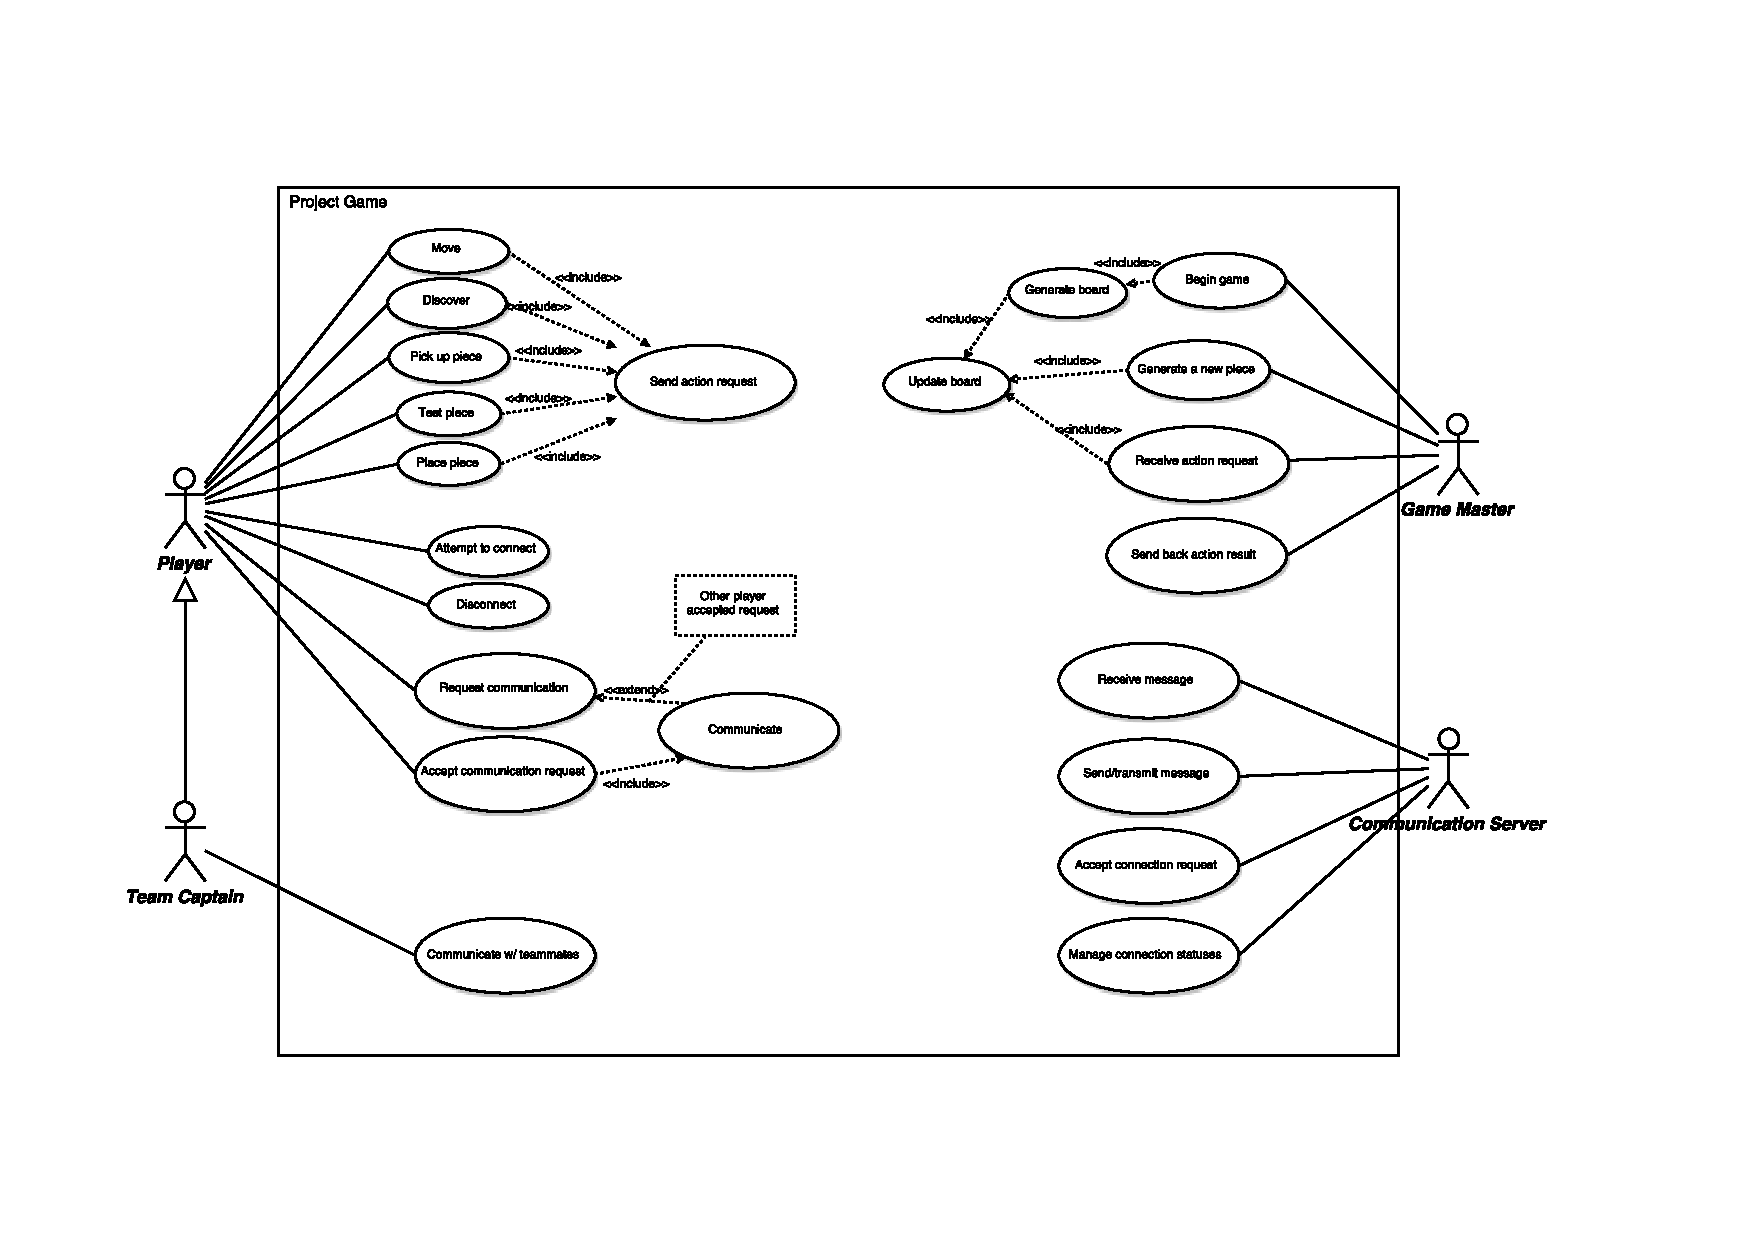
\includegraphics{../res/usecase}
}
\FloatBarrier

\hspace*{-4cm}
\begin{longtable}{|p{.20\textwidth}|p{.03\textwidth}|p{.2\textwidth}|p{.7\textwidth}|}
\caption{Przypadki użycia}
\\
\hline
Aktor 
& Lp 
& Nazwa 
& Opis 
\\ \hline
\endhead
\hline
\endfoot
\multirow{11}{.20\textwidth}{Gracz/Kapitan Drużyny} 
& 1 
& Move 
& Rusz graczem w kierunku góra/dół/lewo/prawo. Aby ruch został zrealizowany, Game Master musi zostać powiadomiony o chęci wykonania tego ruchu i go zatwierdzić (patrz \textit{\# 6 Send action request}). 
\\ \cline{2-4}
& 2 
& Discover 
& Odkryj zawartość otaczających pól oraz poznaj ich odległości od najbliższego zadania. Aby akcja została zrealizowana, musi zostać wykonany \textit{\# 6 Send action request}.
\\ \cline{2-4}
& 3 
& Pick up piece 
& Podnieś zadanie z pola, na którym stoisz. Jeśli gracz stoi na polu z zadaniem, zadanie znika z planszy; w przeciwnym przypadku nic się nie dzieje. Akcja musi zostać zatwierdzona przez Mistrza Gry (patrz \textit{\# 6 Send action request}).
\\ \cline{2-4}
& 4 
& Test piece 
& Sprawdź, czy zadanie jest użyteczne. Jeśli jest bezużyteczne, zostaje wyrzucone. Akcja musi zostać zatwierdzona przez Mistrza Gry (patrz \textit{\# 6 Send action request}).
\\ \cline{2-4}
& 5 
& Place piece 
& Użyj zadania do osiągnięcia celu, na którym stoisz. Jeśli zadanie nie było użyteczne, nie dzieje się nic. Jeśli zadanie było użyteczne, odkrywa cel jako osiągnięty i informuje, czy był to cel służący do zrealizowania projektu. Akcja musi zostać zatwierdzona przez Mistrza Gry (patrz \textit{\# 6 Send action request}). 
\\ \cline{2-4}
& 6 
& Send action request 
& Wyślij zlecenie wykonania akcji (dowolnego przypadku użycia z przedziału 1-5) przez gracza do Mistrza Gry, by mógł potwierdzić poprawność operacji oraz zaktualizować planszę. Wykonywane bez wywołania przez gracza w momencie zlecenia dowolnej z akcji 1-5. Gracz nie posiada żadnych danych poza tymi, które są mu znane. Stąd każda akcja musi być zatwierdzona przez GM, który odsyła zaktualizowaną planszę po każdej zmianie. To zapobiega kolizjom, desynchronizacji i próbom hackowania gry.
\\ \cline{2-4}
& 7 
& Attempt to connect 
& Spróbuj połączyć się z serwerem gry. W wypadku błędu gracz będzie próbował aż do skutku bądź osiągnięcia limitu prób. Potem dołączy do aktualnego stanu gry (powodzenie) lub się wyłączy (niepowodzenie).
\\ \cline{2-4}
& 8 
& Disconnect 
& Rozłącz się z serwerem gry (opuść grę). Natychmiast po tym wyłącza aplikację gracza. Gracz rozłącza się z własnej woli jedynie w przypadku zakończenia gry, chyba że pewna implementacja sztucznej inteligencji w przyszłości będzie zamierzenie rozłączać gracza.
\\ \cline{2-4}
& 9 
& Request communication 
& Wyślij do innego gracza prośbę o rozpoczęcie korespondencji. Skutkuje otwarciem kanału komunikacji między graczami w wypadku zaakceptowania prośby; w przypadku odrzucenia - informacja o tym; w przypadku braku odpowiedzi, po upływie określonego czasu - równoznaczne z odrzuceniem. Od tego momentu gracze mogą fizycznie komunikować się ze sobą.
\\ \cline{2-4}
& 10 
& Accept communication request 
& Zaakceptuj prośbę komunikacji od innego gracza. Otwiera kanał komunikacji między graczami.
\\ \cline{2-4}
& 11 
& Communicate 
& Komunikuj się z innym graczem z drużyny. Wyślij/przeczytaj wiadomość od innego gracza. Wymaga zaakceptowania prośby o komunikację przez docelowego członka drużyny (\# 10).
\\ \hline
Kapitan Drużyny 
& 12 
& Communicate with teammates 
& Komunikuj się z innym członkiem drużyny. Kapitan drużyny ma większe kompetencje od zwykłego gracza i nie musi prosić o komunikację. Automatycznie otwiera dwustronne połączenie do komunikacji między kapitanem a docelowym graczem. 
\\ \hline
\multirow{6}{.20\textwidth}{Game Master}
& 13
& Begin game
& Wyzwala akcję generowania planszy (\# 14). Ustawia stan gry na rozpoczęty. Informuje o tym graczy za pośrednictwem serwera komunikacji. 
\\ \cline{2-4}
& 14
& Generate board
& Generuje planszę po raz pierwszy według podanych w pliku konfiguracyjnym lub w programie danych wejściowych. Wymusza aktualizację planszy i powiadomienie o tym graczy (akcja \# 17).
\\ \cline{2-4}
& 15
& Generate a new piece
& Generuje nowy element \textit{piece} na planszy w obszarze \textit{task area}. Wymusza aktualizację planszy (\# 17).
\\ \cline{2-4}
& 16
& Receive action request
& Odbiera zlecenie wykonania akcji przez gracza (wysłane przez \textit{\# 6 Send action request}). Wykonanie zleconej akcji wymusza aktualizację planszy (\# 17) oraz odesłanie informacji o powodzeniu akcji (\# 18).
\\ \cline{2-4}
& 17
& Update board
& Wprowadza zmiany w planszy i rozsyła odpowiednie informacje o stanie planszy przeznaczone dla graczy.
\\ \cline{2-4}
& 18
& Send back action result
& Odsyła informację o powodzeniu zleconej akcji (odebranej w \# 16).
\\ \hline
\multirow{4}{.20\textwidth}{Communication Server}
& 19
& Receive message
& Odbiera wiadomość będącą na wejściu danego połączenia.
\\ \cline{2-4}
& 20
& Send/transmit message
& Przekierowuje odebraną wcześniej wiadomość (\# 19) do odpowiedniego odbiorcy lub wysyła własny komunikat.
\\ \cline{2-4}
& 21
& Accept connection request
& Akceptuje próbę połączenia przez danego klienta.
\\ \cline{2-4}
& 22
& Manage connection statuses
& Kontroluj stany połączeń. Tworzy nowe tunele dla konwersacji między graczami. Zamyka tunele zakończonych konwersacji. Sprawdza i informuje o nagłych rozłączeniach.
\\ \hline
\end{longtable}
\FloatBarrier

\begin{longtable}[!h]{|p{.20\textwidth}|p{.80\textwidth}|}
\caption{Aktorzy korzystający z systemu}
\\ \hline
Nazwa 
& Opis 
\\ \hline
Gracz 
& Gracz uczestniczący w rozgrywce. Jest programem uruchamianym automatycznie na potrzeby gry. 
\\ \hline
Kapitan Drużyny 
& Wyróżniony gracz, który może bez wysyłania prośby komunikować się z innymi graczami z drużyny. Każda drużyna ma dokładnie jednego kapitana. 
\\ \hline
Game Master
& Aplikacja kontrolująca przebieg gry. Generuje planszę, przekazuje informacje o niej graczom, aktualizuje ją i decyduje o rozpoczęciu i zakończeniu rozgrywki.
\\ \hline
Communication Server
& Aplikacja służąca do ustanowienia komunikacji między graczami i Game Masterem. Jej jedynym celem jest przesyłanie danych i zarządzanie połączeniami.
\\ \hline
\end{longtable}
\FloatBarrier

\subsection{Wymagania niefunkcjonalne}
\par
Żadne wymagania niefunkcjonalne nie zostały określone dla tego projektu.

\subsection{Architektura rozwiązania}
\par
Program zostanie zaimplementowany w strukturze klient-serwer, gdzie klientami będą poszczególni gracze korzystający z aplikacji klienckiej (możliwe będzie korzystanie z jednej maszyny/aplikacji przez kilku graczy jednocześnie z opcją podziału ekranu). Po stronie serwera działać będzie serwer komunikacji oraz jednostka Mistrza Gry.
\par
Wszelka komunikacja gracz-gracz oraz gracz-Mistrz Gry będzie odbywać się za pośrednictwem serwera komunikacji, nawet w wypadku skonfigurowania całego systemu lokalnie na jednej maszynie.

\begin{figure}[!h]
\caption{Architektura systemu}
\resizebox{\textwidth}{!}
{
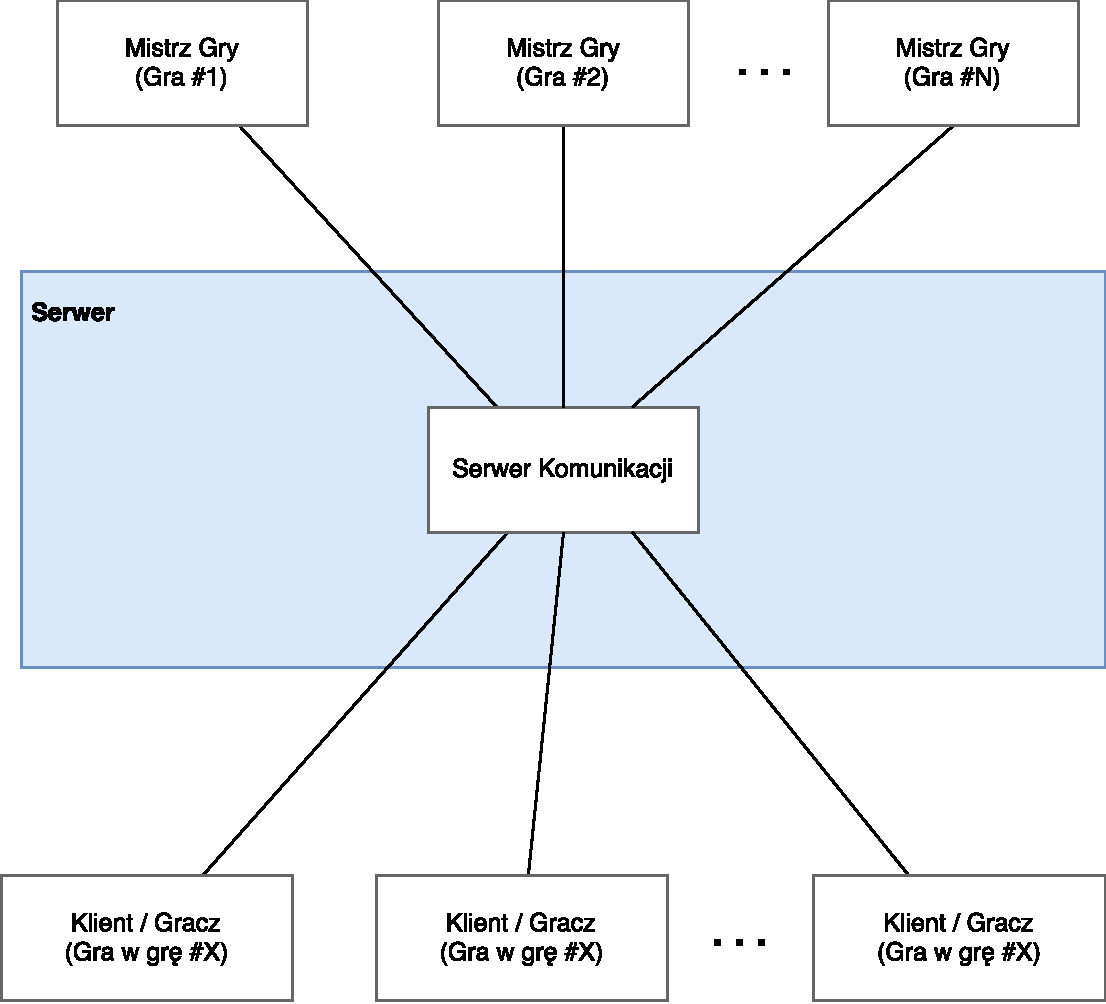
\includegraphics{../res/architecture}
}
\end{figure}
\FloatBarrier

\par
Zależności między obiektami powinny zachodzić jak na poniższym diagramie klas.

\begin{sidewaysfigure}[!h]
\caption{Diagram klas}
\hspace*{-4cm}
\resizebox{1.4\textheight}{!}
{
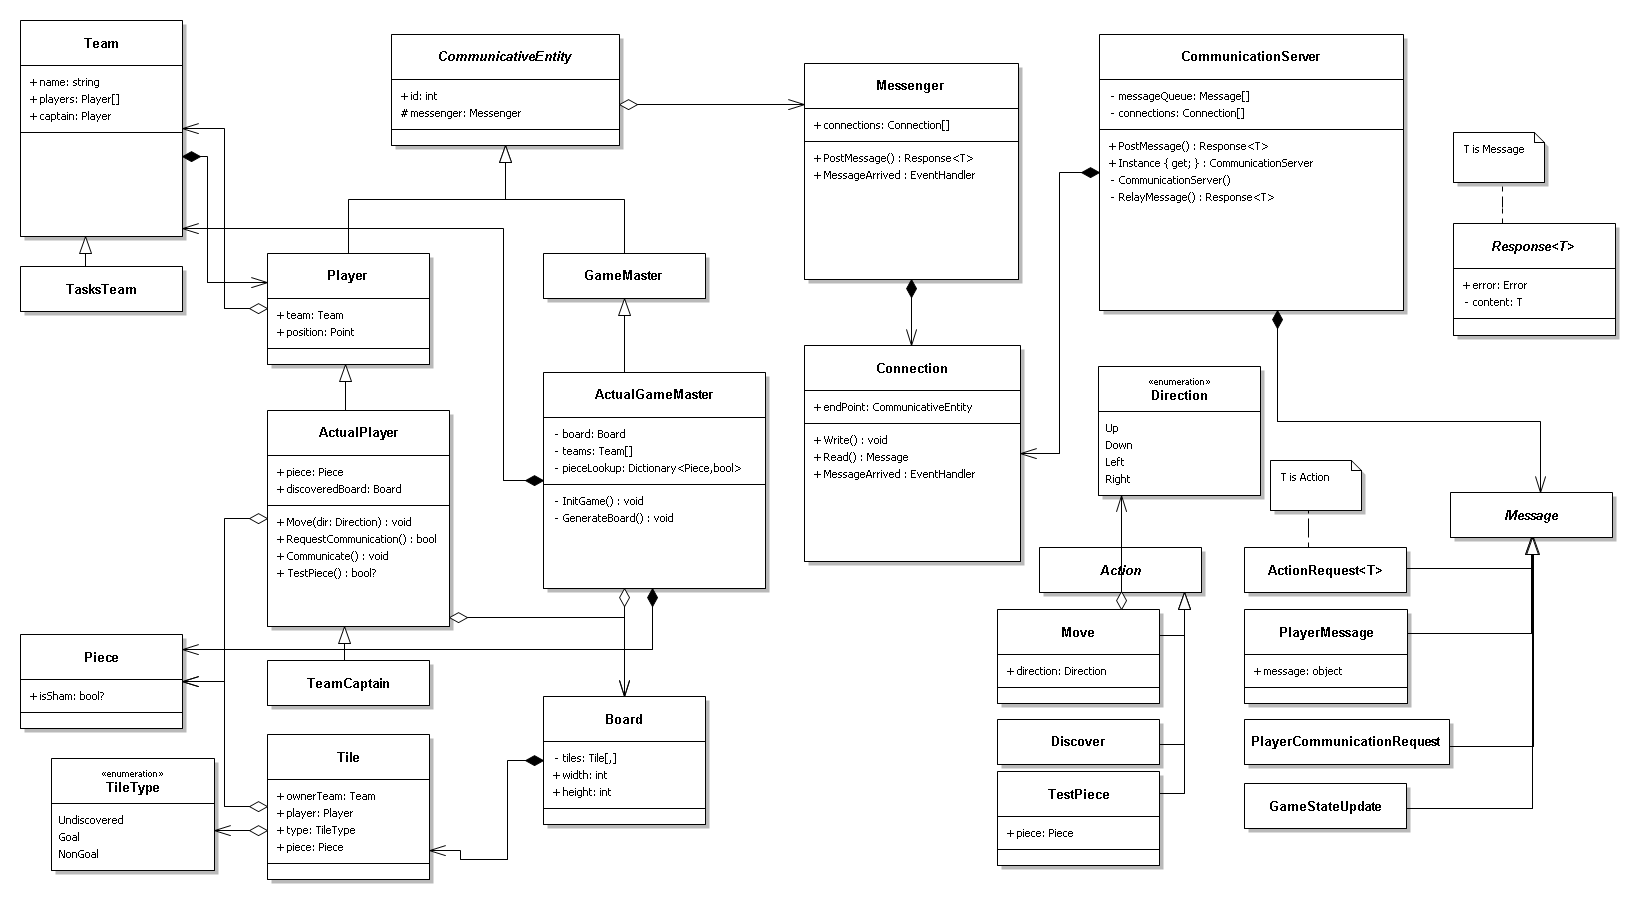
\includegraphics{../res/class_diagram}
}
\end{sidewaysfigure}
\FloatBarrier

\subsection{Opis obiektów}

\begin{description}
	\item[Player] Podstawowe informacje o graczu: drużyna, pozycja na planszy.

	\item[GameMaster] Reprezentacja mistrza gry.

	\item[ActualPlayer] Bieżący użytkownik systemu, jeśli jest on graczem. Posiada operacje wykonywania ruchów i akcji w grze oraz komunikacji z innymi graczami. Przechowuje zdobyte informacje o stanie gry (planszę) oraz o zadaniu, jeśli jakieś znalazł w trakcie gry.

	\item[ActualGameMaster] Bieżący użytkownik systemu, jeśli jest on mistrzem gry. Posiada operacje inicjalizacji gry i generowania planszy. Przechowuje pełną informację o planszy i stanie gry oraz o tym, które zadania są użyteczne, a które nie.

	\item[Team] Drużyna. Są dwie faktyczne drużyna oraz jedna sztuczna, która jest „właścicielem” pól w obszarze zadań.

	\item[Board] Plansza, czyli stan gry --- faktyczny (w przypadku mistrza gry) lub widziany przez gracza.

	\item[Field] Pojedyncze pole na planszy. Posiada odwołanie do drużyny-właściciela; w przypadku pola w obszarze celów będzie to prawdziwa drużyna, a w przypadku pola w obszarze zadań --- instancja TasksTeam. Pole posiada informację o graczu, który na nim stoi. Ponadto dla pól w obszarze zadań jest informacja o zadaniu, które może się znajdować na danym polu, a dla pól w obszarze celów informacja, czy na polu znajduje się cel (o ile użytkownik to wie).

	\item[Piece] Zadanie. Może być użyteczne lub nie (użytkownik może nie wiedzieć).

	\item[Action] Akcja wykonywana przez gracza, taka jak ruch, test zadania, rozpoczęcie komunikacji z innym graczem.

	\item[CommunicativeEntity] Użytkownik systemu mogący komunikować się z innymi użytkownikami. Do komunikacji używa instancji klasy Messenger.

	\item[Messenger] Obiekt wykorzystywany przez użytkownika do komunikacji z innymi. Umożliwia wysyłanie komunikatów i reagowanie na komunikaty przychodzące. Utrzymuje listę połączeń do innych użytkowników (tunelowanych przez serwer komunikacji).

	\item[Message] Komunikat nadawany lub odbierany przez użytkownika. Wyróżnia się kilka rodzajów:
		\begin{description}
			\item[ActionRequest<T>] Żądanie zatwierdzenia pewnej akcji gracza, wysyłane przez niego do mistrza gry.
			\item[PlayerMessage] Wiadomość od jednego gracza do drugiego.
			\item[PlayerCommunicationRequest] Prośba o rozpoczęcie wymiany informacji, kierowana przez jednego gracza do drugiego.
			\item[GameStateUpdate] Informacja (być może częściowa) o zmianach stanu gry (czyli o zmianach na planszy), wysyłana przez mistrza gry do gracza (np. wskutek wykonania przez gracza poprawnej akcji).
		\end{description}

	\item[Connection] Połączenie z użytkownikiem. Obiekt odpowiadający za komunikację niskopoziomową.

	\item[ComunicationServer] Serwer komunikacji przekazujący wiadomości między użytkownikami. Singleton. Posiada listę bezpośrednich połączeń do użytkowników. Nadchodzące wiadomości są gromadzone w kolejce, z której serwer je pobiera i przekazuje do adresatów.
\end{description}

\subsection{System komunikacji}

\subsubsection{Mechanizm}
\par
Wszelka komunikacja może występować w następujących płaszczyznach:
\begin{description}
\item[Mistrz Gry - Serwer Komunikacji] Służy ustanowieniu połączenia. Ponadto serwer komunikacji informuje mistrza gry o zaburzeniach toku gry w postaci rozłączeń.
\item[Gracz - Serwer Komunikacji] Służy ustanowieniu i utrzymaniu połączenia.
\item[Gracz - Mistrz Gry] Mistrz Gry informuje graczy o zmianach w układzie planszy, przekazuje im konsekwencje ich działań oraz o statusie gry. Gracze zlecają Mistrzowi Gry wykonanie operacji na rzecz gracza.
\item[Gracz - Gracz] Gracze mogą komunikować się między sobą, by przekazać informacje o planszy i stanie gry z ich perspektywy.
\end{description}

\par
Niezależnie od płaszczyzny, \textbf{serwer komunikacji} zawsze jest ogniwem w drodze przekazywania komunikatów. Albo on sam komunikuje się (MG - Serwer lub Gracz - Serwer), albo przekazuje komunikaty między graczami a mistrzem gry lub graczami a graczami. Nie istnieją połączenia bezpośrednie, omijające \textbf{serwer komunikacji}.
\par
Pomimo tego, że serwer komunikacji pośredniczy w każdej wymianie informacji, każda jednostka zdolna komunikować się (\textit{CommunicativeEntity}) posiada moduł (\textit{Messenger}), który wykonuje wszystkie działania potrzebne do komunikacji. Z punktu widzenia takiej jednostki komunikacja jest bezpośrednia, ponieważ dla każdej pary jednostek komunikujących się \textbf{serwer komunikacji} tworzy połączenie w postaci wirtualnego tunelu. Tunel posiada dwa punkty wejścia/wyjścia, to jest \textit{Messengery} dwóch jednostek komunikujących się ze sobą. Z zewnątrz nie widać żadnych mechanizmów wewnętrznych, można jedynie pisać do tunelu i odczytywać wiadomości z niego. W rzeczywistości jednak tunel prowadzi przez \textbf{serwer komunikacji}, który przekazuje wiadomości na bieżąco do \textit{Messengerów}.

\subsubsection{Protokół}
\par
Wszystkie wiadomości zostają przekonwertowane na format JSON. Wybór ten jest motywowany niezależnością od języka programowania, powszechnością parserów oraz choćby tym, że format JSON jest bardziej zwięzły niż XML. Następnie łańcuch znaków jest pakowany w pakiety TCP/IP i transmitowany. TCP, mimo że powolniejszy niż UDP, bo wymaga potwierdzeń i uwzględnia retransmisję, jest wygodniejszy w użyciu. Ponadto prędkość UDP nie zostałaby w pełni wykorzystana, ponieważ gra nie jest na tyle złożona.
\par
Przykładowy komunikat - zlecenie ruchu o jedno pole w górę - wygląda następująco:
\begin{lstlisting}
{ 
	"type":"ActionRequest<Move>",
	"data":{
		"dir":"0"
	}
}
\end{lstlisting}

\subsubsection{Scenariusze wymiany komunikatów}

\paragraph{Akcja gracza}

Sytuacja, gdy gracz zamierza wykonać jakąś akcję, taką jak: przemieszczenie się, sprawdzenie lub wykorzystanie posiadanego zadania, sprawdzenie sąsiadujących pól.
Gracz wysyła żądanie do mistrza gry. Mistrz gry odsyła wynik akcji lub informację, że jest nieprawidłowa.

\begin{figure}[!h]
	\centering
	\caption{Diagram sekwencji}
\resizebox{0.9\textwidth}{!}{
	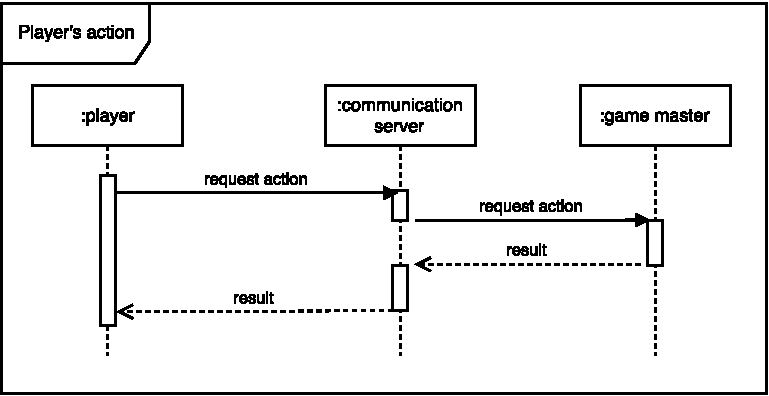
\includegraphics{../res/p_gm_action_generic}
}
\end{figure}
\FloatBarrier

\paragraph{Komunikacja graczy}

Sytuacja, gdy jeden gracz chce wymienić informacje z drugim. Pierwszy gracz musi zapytać drugiego o pozwolenie. Musi w tym pośredniczyć mistrz gry, ponieważ jest to traktowane jako rodzaj akcji. Drugi gracz może prośbę zaakceptować lub nie. W przypadku akceptacji obie strony przesyłają sobie nawzajem informacje.

\begin{figure}[!h]
	\centering
	\caption{Diagram sekwencji}
\resizebox{0.9\textwidth}{!}{
	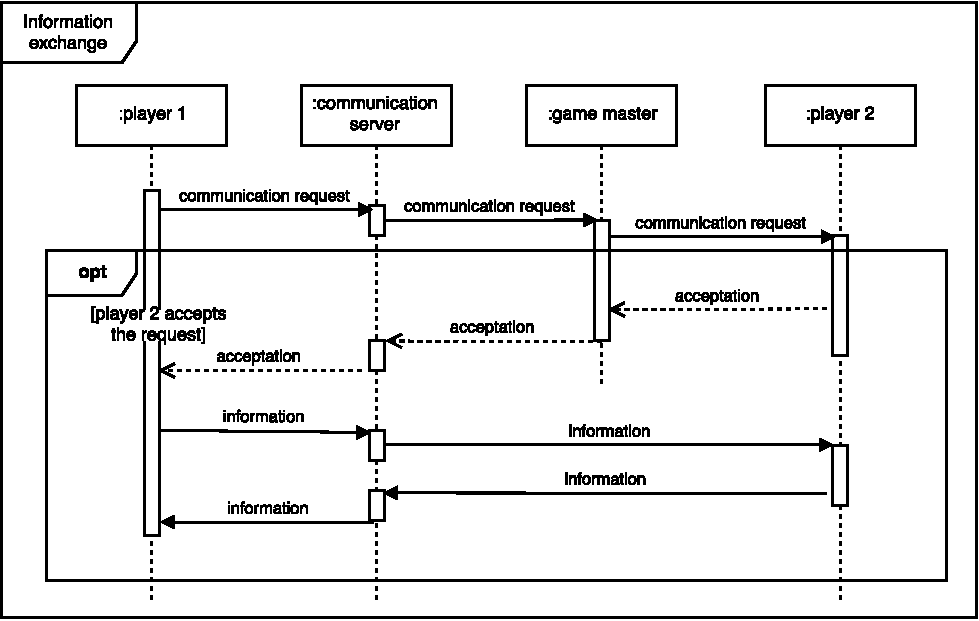
\includegraphics{../res/pp_gm_comm}
}
\end{figure}
\FloatBarrier
\par

\paragraph{Komunikacja kierownika z zespołem}

Sytuacja, gdy kierownik zespołu chce wymienić informacje innym członkiem drużyny. Kierownik nie musi pytać o pozwolenie.

\begin{figure}[!h]
	\centering
	\caption{Diagram sekwencji}
\resizebox{0.9\textwidth}{!}{
	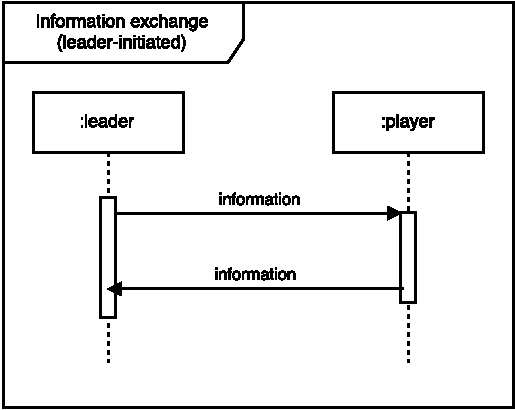
\includegraphics{../res/p_tl_comm}
}
\end{figure}
\FloatBarrier
\par

\paragraph{Rozgłaszanie komunikatów}

Scenariusz, w którm mistrz gry musi o czymś powiadomić wszystkich graczy, np. o zakończeniu gry. Do każdego gracza jest wysyłana taka sama wiadomość.

\begin{figure}[!h]
	\centering
	\caption{Diagram sekwencji}
\resizebox{0.9\textwidth}{!}{
	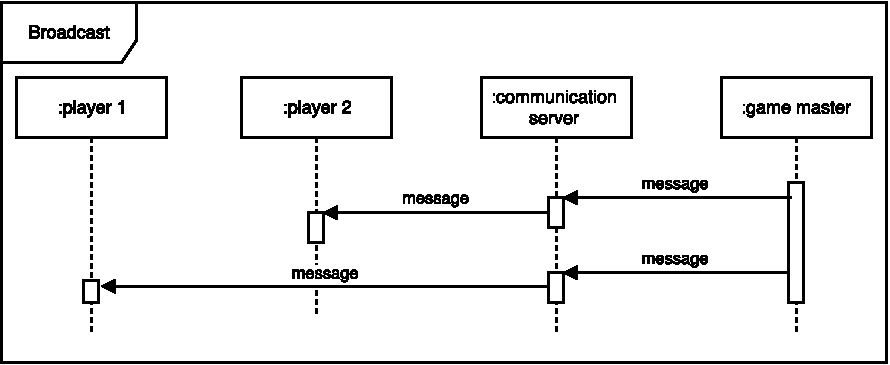
\includegraphics{../res/broadcast}
}
\end{figure}
\FloatBarrier

\paragraph{Łączenie z serwerem}

Łączenie jest dokonywane przez graczy i mistrza gry tuż po wystartowaniu. W przypadku niepowodzenia podejmowane są kolejne próby aż do wyczerpania ich limitu. Udana próba połączenia kończy się odbiorem potwierdzenia od serwera.

\begin{figure}[!h]
	\centering
	\resizebox{0.9\textwidth}{!}{
	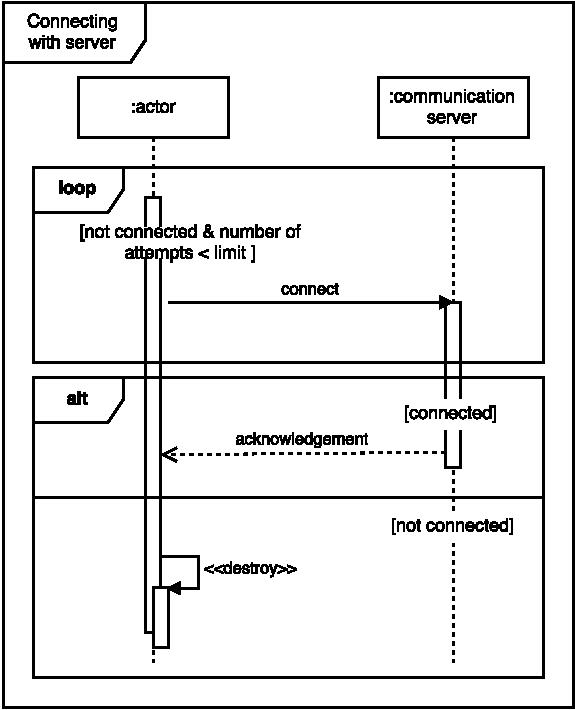
\includegraphics{../res/srv_conn}
}
	\caption{Diagram sekwencji}
\end{figure}

\subsection{Użytkowanie aplikacji}

\subsubsection{Uruchomienie i konfiguracja}
\par
Grę uruchamia się za pomocą prostej aplikacji administratora, pozwalającej ustalić konfigurację rozgrywki i uruchomić ją, a następnie za jej pomocą śledzić jej przebieg. Poza tą aplikacją konfigurację można również wprowadzić edytując plik konfiguracyjny i uruchamiając grę bezpośrednio, ale jest to metoda mniej user-friendly.

\subsubsection{Przebieg rozgrywki}

\subsubsection{Wyjątki}
\par
Podczas rozgrywki może zdarzyć się wiele nieprzewidzianych błędów. Wynikają one przede wszystkim z wadliwych połączeń. Poniżej opisane są akcje podejmowane w wypadku możliwych scenariuszy błędów.

\paragraph{Utrata łączności z graczem}
\par
W momencie, gdy serwer stwierdzi brak połączenia z graczem, podejmie zdefiniowaną w czasie konfiguracji akcję. Możliwe będą:
\begin{enumerate}
\item Zakończenie gry bez podania wyniku
\item Zakończenie gry, przegrywa drużyna, która straciła gracza
\item Kontynuacja gry bez rozłączonego gracza (jeśli zostanie 0 graczy w danej drużynie, koniec gry - drużyna przegrywa walkowerem lub gra kończy się bez podania wyniku)
\item Próba uruchomienia i dołączenia nowego gracza, by kontynuował w miejscu rozłączonego gracza (w przypadku kilku nieudanych prób dołączenia można zakończyć grę z błędem)
\end{enumerate}

\paragraph{Utrata łączności z serwerem}
\par
Jeśli to mistrz gry traci łączność z serwerem, to serwer informuje o tym graczy, którzy sami powinni się rozłączyć. Po chwili ucina pozostałe połączenia i się wyłącza. W tym czasie mistrz gry wyłącza się. Aplikacja gry zwraca komunikat o błędzie i proponuje ponowne uruchomienie.
\par
Jeśli gracz traci łączność z serwerem, próbuje połączyć się ponownie z maksymalną liczbą prób określoną podczas konfiguracji. Jeśli mu się to nie uda, wyłącza się.

\paragraph{Utrata łączności z mistrzem gry}
\par
W przypadku utraty łączności z mistrzem gry patrz par. \textit{1.7.3.2 Utrata łączności z serwerem} - akapit 1.


\end{document}
